\section{Experiments and Results}

When a shopper goes shopping in a retail store or surfs on app for purchasing merchandises, 
he/she generally has merchandise list either in the form of notes or on top of his mind. 
In general the merchandise list of the regular shoppers happens to be huge and has hidden pattern. 
The problem on hand uses customer and his/her transaction data over time and attempts to predict 
the next basket of the customer leveraging his/her past purchased merchandises.This will provide 
very smooth and delightful shopping experience for the shoppers.

\subsection{Experiments}
When a shopper goes shopping in a retail store or surfs on app for purchasing merchandises, 
he/she generally has merchandise list either in the form of notes or on top of his mind. 
In general the merchandise list of the regular shoppers happens to be huge and has hidden pattern. 
The problem on hand uses customer and his/her transaction data over time and attempts to predict 
the next basket of the customer leveraging his/her past purchased merchandises.This will provide 
very smooth and delightful shopping experience for the shoppers.
When a shopper goes shopping in a retail store or surfs on app for purchasing merchandises, 
he/she generally has merchandise list either in the form of notes or on top of his mind. 
In general the merchandise list of the regular shoppers happens to be huge and has hidden pattern. 
The problem on hand uses customer and his/her transaction data over time and attempts to predict 
the next basket of the customer leveraging his/her past purchased merchandises.This will provide 
very smooth and delightful shopping experience for the shoppers. It is meant to acheive three major 
objectives: - Revenue Enablement: A SmartList that predicts what merchandise a customer is likely to 
purchase during his next visit Relevance: The SmartList prediction is expected to achieve a 
satisfactory accuracy level so that the customer finds the SmartList relevant User Experience: 
The size of a SmartList should be manageable so as not to overwhelm the customers with too many 
merchandises. Build a framework to predict the next basket for each customer.
When a shopper goes shopping in a retail store or surfs on app for purchasing merchandises, 
he/she generally has merchandise list either in the form of notes or on top of his mind. 

\begin{figure}[t]
  \centering 
  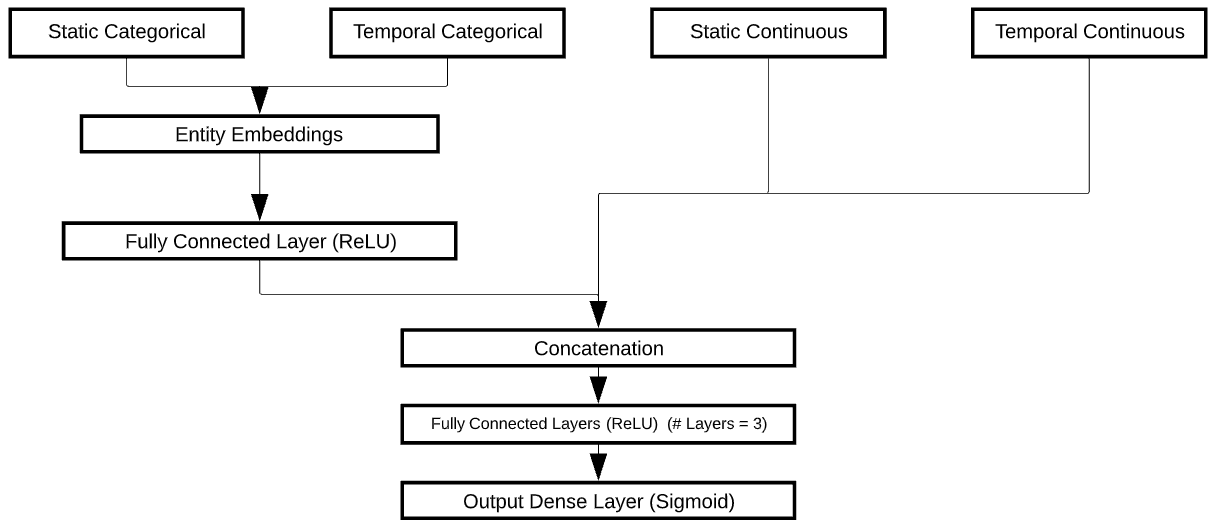
\includegraphics[width=3.3in]{img/MLP.png} 
  \caption{MLP Architecture} 
  \label{fig:MLP} 
\end{figure}

In general the merchandise list of the regular shoppers happens to be huge and has hidden pattern. 
The problem on hand uses customer and his/her transaction data over time and attempts to predict 
the next basket of the customer leveraging his/her past purchased merchandises.This will provide 
very smooth and delightful shopping experience for the shoppers. It is meant to acheive three major 
objectives: - Revenue Enablement: A SmartList that predicts what merchandise a customer is likely to 
purchase during his next visit Relevance: The SmartList prediction is expected to achieve a 
satisfactory accuracy level so that the customer finds the SmartList relevant User Experience: 
The size of a SmartList should be manageable so as not to overwhelm the customers with too many 
merchandises. Build a framework to predict the next basket for each customer.
When a shopper goes shopping in a retail store or surfs on app for purchasing merchandises, 
he/she generally has merchandise list either in the form of notes or on top of his mind. 

\subsection{Evaluation}

In general the merchandise list of the regular shoppers happens to be huge and has hidden pattern. 
The problem on hand uses customer and his/her transaction data over time and attempts to predict 
the next basket of the customer leveraging his/her past purchased merchandises.This will provide 
very smooth and delightful shopping experience for the shoppers. It is meant to acheive three major 
objectives: - Revenue Enablement: A SmartList that predicts what merchandise a customer is likely to 
purchase during his next visit Relevance: The SmartList prediction is expected to achieve a 
satisfactory accuracy level so that the customer finds the SmartList relevant User Experience: 
The size of a SmartList should be manageable so as not to overwhelm the customers with too many 
merchandises. Build a framework to predict the next basket for each customer.
When a shopper goes shopping in a retail store or surfs on app for purchasing merchandises, 
he/she generally has merchandise list either in the form of notes or on top of his mind. 
In general the merchandise list of the regular shoppers happens to be huge and has hidden pattern. 
The problem on hand uses customer and his/her transaction data over time and attempts to predict 
the next basket of the customer leveraging his/her past purchased merchandises.This will provide 
very smooth and delightful shopping experience for the shoppers. It is meant to acheive three major 
objectives: - Revenue Enablement: A SmartList that predicts what merchandise a customer is likely to 
purchase during his next visit Relevance: The SmartList prediction is expected to achieve a 
satisfactory accuracy level so that the customer finds the SmartList relevant User Experience: 
The size of a SmartList should be manageable so as not to overwhelm the customers with too many 
merchandises. Build a framework to predict the next basket for each customer.
When a shopper goes shopping in a retail store or surfs on app for purchasing merchandises, 
he/she generally has merchandise list either in the form of notes or on top of his mind. 

\subsection{Results}

In general the merchandise list of the regular shoppers happens to be huge and has hidden pattern. 
The problem on hand uses customer and his/her transaction data over time and attempts to predict 
the next basket of the customer leveraging his/her past purchased merchandises.This will provide 
very smooth and delightful shopping experience for the shoppers. It is meant to acheive three major 
objectives: - Revenue Enablement: A SmartList that predicts what merchandise a customer is likely to 
purchase during his next visit Relevance: The SmartList prediction is expected to achieve a 
satisfactory accuracy level so that the customer finds the SmartList relevant User Experience: 
The size of a SmartList should be manageable so as not to overwhelm the customers with too many 
merchandises. Build a framework to predict the next basket for each customer.
When a shopper goes shopping in a retail store or surfs on app for purchasing merchandises, 
he/she generally has merchandise list either in the form of notes or on top of his mind. 
In general the merchandise list of the regular shoppers happens to be huge and has hidden pattern. 

\begin{figure}[t]
  \centering 
  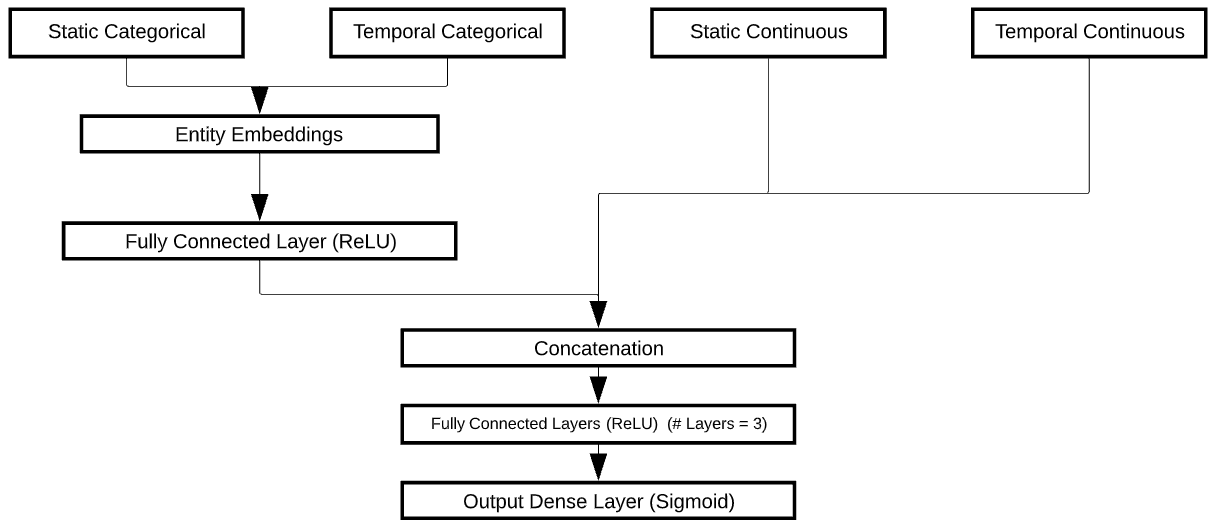
\includegraphics[width=3.3in]{img/MLP.png} 
  \caption{MLP Architecture} 
  \label{fig:MLP} 
\end{figure}

The problem on hand uses customer and his/her transaction data over time and attempts to predict 
the next basket of the customer leveraging his/her past purchased merchandises.This will provide 
very smooth and delightful shopping experience for the shoppers. It is meant to acheive three major 
objectives: - Revenue Enablement: A SmartList that predicts what merchandise a customer is likely to 
purchase during his next visit Relevance: The SmartList prediction is expected to achieve a 
satisfactory accuracy level so that the customer finds the SmartList relevant User Experience: 
The size of a SmartList should be manageable so as not to overwhelm the customers with too many 
merchandises. Build a framework to predict the next basket for each customer.
When a shopper goes shopping in a retail store or surfs on app for purchasing merchandises, 
he/she generally has merchandise list either in the form of notes or on top of his mind. 
The problem on hand uses customer and his/her transaction data over time and attempts to predict 
the next basket of the customer leveraging his/her past purchased merchandises.This will provide 
very smooth and delightful shopping experience for the shoppers. It is meant to acheive three major 
objectives: - Revenue Enablement: A SmartList that predicts what merchandise a customer is likely to 
purchase during his next visit Relevance: The SmartList prediction is expected to achieve a 
satisfactory accuracy level so that the customer finds the SmartList relevant User Experience: 
The size of a SmartList should be manageable so as not to overwhelm the customers with too many 
merchandises. Build a framework to predict the next basket for each customer.
When a shopper goes shopping in a retail store or surfs on app for purchasing merchandises, 
he/she generally has merchandise list either in the form of notes or on top of his mind. 

\begin{figure}[t]
  \centering 
  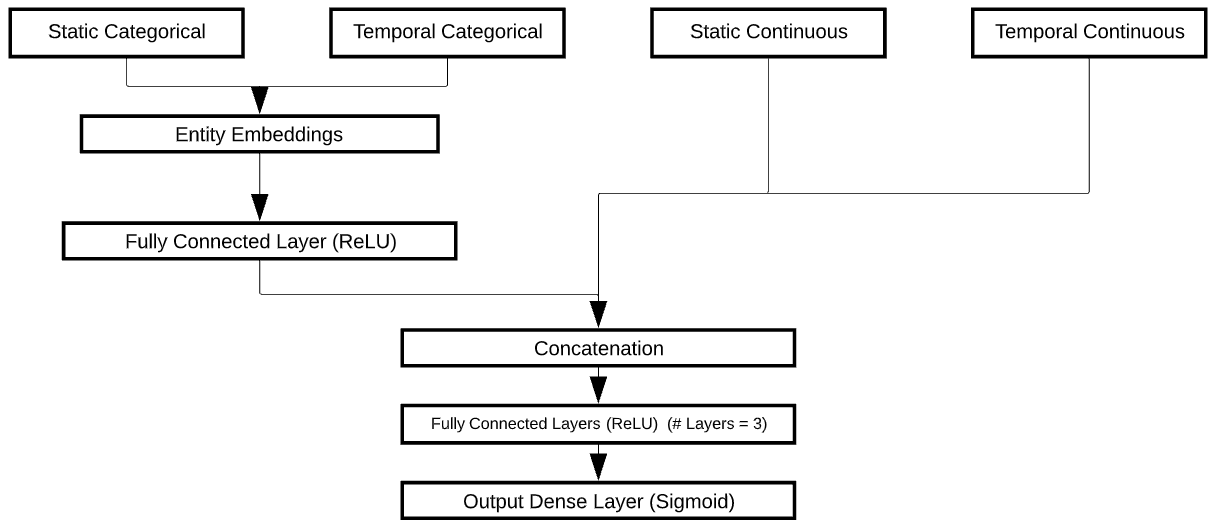
\includegraphics[width=3.3in]{img/MLP.png} 
  \caption{MLP Architecture} 
  \label{fig:MLP} 
\end{figure}

The problem on hand uses customer and his/her transaction data over time and attempts to predict 
the next basket of the customer leveraging his/her past purchased merchandises.This will provide 
very smooth and delightful shopping experience for the shoppers. It is meant to acheive three major 
objectives: - Revenue Enablement: A SmartList that predicts what merchandise a customer is likely to 
purchase during his next visit Relevance: The SmartList prediction is expected to achieve a 
satisfactory accuracy level so that the customer finds the SmartList relevant User Experience: 
The size of a SmartList should be manageable so as not to overwhelm the customers with too many 
merchandises. Build a framework to predict the next basket for each customer.
When a shopper goes shopping in a retail store or surfs on app for purchasing merchandises, 
he/she generally has merchandise list either in the form of notes or on top of his mind. 
The problem on hand uses customer and his/her transaction data over time and attempts to predict 
the next basket of the customer leveraging his/her past purchased merchandises.This will provide 
very smooth and delightful shopping experience for the shoppers. It is meant to acheive three major 
objectives: - Revenue Enablement: A SmartList that predicts what merchandise a customer is likely to 
purchase during his next visit Relevance: The SmartList prediction is expected to achieve a 
satisfactory accuracy level so that the customer finds the SmartList relevant User Experience: 
The size of a SmartList should be manageable so as not to overwhelm the customers with too many 
merchandises.
